\documentclass[a4paper,fleqn,twoside,11pt]{article}

%%%%%%%%%%%%%%%%%%%%


\usepackage[]{geometry}
\usepackage[latin1]{inputenc}
\usepackage[UKenglish]{babel}
\usepackage[UKenglish]{isodate}
\usepackage{amsmath}
\usepackage{amsfonts}
\usepackage{amssymb}
\usepackage{amsthm}
\usepackage{graphicx}
\usepackage{chngpage}
\usepackage{calc}
\PassOptionsToPackage{hyphens}{url}
\usepackage{hyperref}
\usepackage[nameinlink]{cleveref}
\usepackage{fancyhdr}
\usepackage{titletoc}
\usepackage[explicit]{titlesec}
\usepackage{natbib}
\usepackage[dvipsnames]{xcolor}
\usepackage[sc]{mathpazo}
\linespread{1.05} 
\usepackage[T1]{fontenc}
\usepackage{minted}

\hypersetup{
	colorlinks=true,
	linkcolor=black,
	urlcolor=black,
	citecolor=black
}

\setlength{\parindent}{0mm}
\setlength{\parskip}{\medskipamount}
\renewcommand\baselinestretch{1.2}

\cleanlookdateon

\makeatletter
\newcommand{\@assignment}[0]{Assignment}
\newcommand{\assignment}[1]{\renewcommand{\@assignment}{#1}}
\makeatletter

%%%%%%%%%%%%%%%%%%%%%%%%%%%%%%%%%%%%%%%%%%%%%%%%%%%%%%%%%%%%%%%%%%%%%%%%%%%%%%%
%% Project-specific configuration
%%%%%%%%%%%%%%%%%%%%%%%%%%%%%%%%%%%%%%%%%%%%%%%%%%%%%%%%%%%%%%%%%%%%%%%%%%%%%%%

\author{Joe Moore, u1917702}
\title{Wondough Bank Coursework\\(CS263 Cyber Security)}

%%%%%%%%%%%%%%%%%%%%%%%%%%%%%%%%%%%%%%%%%%%%%%%%%%%%%%%%%%%%%%%%%%%%%%%%%%%%%%%


\assignment{Progress report}

%%%%%%%%%%%%%%%%%%%%

\pagestyle{plain}
\renewcommand{\headrulewidth}{0.0pt}

\makeatletter
\fancypagestyle{plain}{
	\fancyhf{}
	\fancyhead[LE]{\thepage}
	\fancyhead[RE]{\textit{\@author}}
	\fancyhead[RO]{\thepage}
	\fancyhead[LO]{\textit{\@title}}
}
\makeatother

\usepackage{minted}
\usepackage[
backgroundcolor = gray!5
, hidealllines=true
]{mdframed}

\surroundwithmdframed{minted}
\usemintedstyle{lovelace}

\setminted[text]{fontsize=\small}
\setminted[java]{fontsize=\small}
\setminted[sql]{fontsize=\small}

%%%%%%%%%%%%%%%%%%%%

\begin{document}

\makeatletter
\begin{titlepage}

\textbf{\Huge \@title} \\
\Large \@assignment \\[1.5cm] 
\Large \textbf{\@author} \\
Department of Computer Science \\
University of Warwick \\

\vfill 

\begin{adjustwidth}{-\oddsidemargin-1in}{-\rightmargin}
    \centering
    
\includegraphics[width=\paperwidth]{../common/line.png}
\end{adjustwidth}

\vspace*{-3.5cm}

\end{titlepage}
\makeatother

\pagestyle{plain}
\tableofcontents

\section{Introduction}

Having penetration tested the Wondough bank website, a number of security flaws were subsequently found. The ten most critical vulnerabilities were then fixed as
well as automated tests devised such that it were possible to entirely ensure the robustness of the new system. Below each of the vulnerabilitiesare otulined alongside
the relevent fix and the tests devised to guarantee the success of my improved system.

\section{Vulnerability: SQL Injection Attack}
\label{sec:background}
\textbf{Description:} The user data of the bank members is stored in a database, and as such upon clicking the login button the bank performs a simple SQL lookup query in order to
determine if the username exists in the database. However this does not make use of \textit{prepared statements} but rather constructs the SQL query using string concatenation.
This allows the user to use the common technique of including an \textit{OR} followed by a comment to finish the line to gain access. This is demonstrated below:
\begin{minted}{text}
   Username inputted: John
\end{minted}
\begin{minted}{sql}
   SQL: SELECT * FROM users WHERE username='John' LIMIT 1;
\end{minted}
\begin{minted}{text}
   Username inputted: blank' OR 1=1;--
\end{minted}
\begin{minted}{sql}
   SQL: SELECT * FROM users WHERE username='blank' OR 1=1;--' LIMIT 1;
\end{minted}
As can be seen in the query generated in the second instance, an entirely new SQL query has been created with the \textbf{- -} used to comment out the rest of the line.
Since 1=1 will always be true, whether the username exists in the database is irrelevant since the statement will return the first user in the database regardless. This is a dangerous
prospect as may allow a hacker access without relevant information and as such needs to be addressed.\\ \\
\textbf{Testing the Vulnerability:} The Vulnerability gives access for all of the following usernames entered:
 
\begin{minted}{text}
   blank' OR 1=1;--
   blank' OR 'x'='x';--
   blank' OR '*;--
   blank' OR TRUE;--
\end{minted}
Where 1 can be replaced with any number as well as 'x' and 'blank' any string. This can also be used to get any value from any table and since tokens are not time dependent, access
to these would allow the hacker to gain full access to an account. This therefore is a serious security flaw.\\ \\
\textbf{Mitigation:} The issue caused by this flaw is purely as a result of using string concatenation to generate the query. The use of sql prepared statements can be implemented in order
to deny such an attack. A prepared statement works by compiling the statement template before later binding values for the parameters of the statement template. As such the statement knows
when the query ends and  the use of ' to signify the end of the username or - - to turn the remainder of the statement to a comment both no longer work. As such the attack no longer works. A
prepared statement works as follows:\\
 
Rather than creating and executing the query as follows:
\begin{minted}{java}
   PreparedStatement stmt = null;
   String query = "SELECT * FROM users WHERE username='"
         + username + "' LIMIT 1;";
   stmt = this.connection.Statement();
   ResultSet rs = stmt.executeQuery(query);
\end{minted}
It is done as follows:
\begin{minted}{java}
   PreparedStatement stmt = null;
   String query = "SELECT * FROM users WHERE username=? LIMIT 1;";
   stmt = this.connection.prepareStatement(query);
   stmt.setString(1, username);
   ResultSet rs = stmt.executeQuery();
\end{minted}
This is the change I made to the \verb|DbConnection.java| file in order to mitigate this attack. Below is the automated test I designed in order to test the changes appropriately extinguished the
vulnerability. Therefore I designed an automated test to run automatically on the startup of the server to check this vulnerability was not a threat. It can be seen at \verb|test1.java|. It
works by calling the get user function with all four examples of SQL injection commands given previously. If none of them return a user then it passes else it fails. Below is the
important check.\begin{minted}{java}
private String runSQLInjection(){
   String[] testSQLInjections = {"blank' OR 1=1;--",
   "blank' OR 'x'='x';--", "blank' OR '*;--", "blank' OR TRUE;--"};
   DbConnection db = Program.getInstance().getDbConnection();
   try {
      for (int i = 0; i <= 3; i++) {
      if (db.getUser(testSQLInjections[i]) instanceof WondoughUser)
         return "FAILED";
      }
   }
   catch (SQLException e) {
      return "FAILED" + e.toString();
   }
   return "PASSED";
}
\end{minted}
This test passed upon starting the server after implementing my fix and as such I consider this vulnerability solved.
\section{Vulnerability: Sending more money than balance}
\label{sec:background}
\textbf{Description:} Upon further penetration testing it was discovered that it was possible 
to send money from the account logged in on to another of a larger amount than the account's balance. This may, upon first glance appear to be a bug rather than
necessarily a vulnerability. However, from the previous section we have displayed proof of concept that it is possible for a hacker to gain access to someone's
account without the relevant information. As such he could feasibly send any amount (even ludicrous sums like \£1 billion) from this bank account at Wondough bank
to his bank account with another bank. His bank likely does not have this issue and he has just granted himself huge amounts of money illegally. \\ \\
\textbf{Testing the Vulnerability:} In order to test this vulnerability I wanted to test to see different things the flaw could enable. It is possible to send
transactions to yourself however I do not see how useful this is as a vulnerability to an attacker. However I then decided to add a new user to the database in order
to carry out further tests. \\ \\
\textbf{Mitigation:} The process of creating a transaction occurs in the \verb|DbConnection| file in the \verb|createTransaction()| procedure. This feature already
includes a check to ensure the amount in the transaction is not negative, as follows:
\begin{minted}{java}
if(amount < 0) {
        return false;
}
\end{minted}
And as such in a similar vein an additonal check was then added which makes use of the \verb|getTransactions(user)| and \verb|getAccountBalance()| functions to retrieve
the user's balance and compare it to the amount. As follows:
\begin{minted}{java}
if(amount > getTransactions(user).getAccountBalance()){
    return false;
}
\end{minted}
This was then tested manually with inputs larger than the balance, which were all not entered as transactions, followed by the balance itself and values lower than it, all of
which the fix permitted. However I then set about automating this testing. The automatic testing seen in \verb|test2.java| creates a new user \textit{testUser}, it then tries
to remove his account balance + 1, which should fail if the fix is correct. It then tries the same with his exact account balance, if this works then the fix is perfect. Since
both these conditions are always fine, this vulnerability has been correctly fixed.
\section{Vulnerability: JavaScript Injection Attack}
\label{sec:background}
\textbf{Description:} A second type of injection attack works on this website. It was possible to enter a JavaScript script into the transaction box. This would be stored by
the database as the description of the transaction. Consequently when the user clicked \textit{List transactions} each transaction would be listed, and as such each description
interpreted in html. This means a description enclosed by \verb|<script></script>| tags will be interpreted as a script and as such executed as the website comes to list the
transactions. This allows a hacker to gain valuable information by printing out session data in a pop up window. This security flaw is exasperated by the fact that all transactions
are viewable to all users. Thus any script injected will affect all users. This is known as a persistent (or stored) vulnerability. Persistent vulnerabilities are more significant
since the malicious script is rendered automatically, therefore there is no requirement to individually target victims or to take them to a third party website.\\ \\
\textbf{Testing the Vulnerability:} To test this vulnerability a series of JavaScript queries were entered as transactions. One of the most dangerous was the following:
\begin{minted}{html}
   <script>alert(document.cookie)</script>
\end{minted}
Once injected upon the selection of \textit{List transactions} this will open a popup window which will display the users token.
\begin{figure}[h]
   \centering
   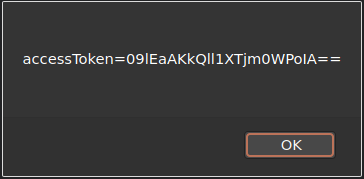
\includegraphics[width=0.5\textwidth]{figs/popup.png}
   \caption{The popup window displayed when a user clicks \textit{List transactions}}
   \label{popup}
\end{figure}\\
git
As can be seen from this figure, this injecton allows a user to display the token. This again being particularly dangerous since the tokens are not time dependent on this website.
Consequently this can be said to be a major security flaw since it has the possibility of allowing a hacker indefinite access to the banking website.\\ \\
\textbf{Mitigation:} 
 

\section{Vulnerability: Multiple users with duplicate usernames}
\label{sec:background}
\textbf{Description:} The fourth vulnerability I discovered was the ability for multiple users to have the same username. This is a fundamental issue. The username of an account
needs to be its unique identifier that allows a program to identify an individual specific user. If we allow multiple users to share a username then what will happen is that
upon one of those users signing in, the program will return the id of the first user in the database with that username. This means that either if they have by chance chosen a
bad and matching password that access to another user's finances could be granted to another. Otherwise it will be impossible for a user to sign in and to access their finances,
which is without doubt a serious issue.\\ \\
\textbf{Testing the Vulnerability:} To test this vulnerability I first uncommented the section of code that creates a new user. This then created the user \textit{test4User}
twice, with passwords \textit{password} and \textit{password2} respectively. I then signed in to the website, as \textit{test4User@wondoughbank.com}, which I was only able to
do using the password \textit{password}, since upon getting the user the program was returning the first instance in the database. Therefore in a real world scenario the second
user with password \textit{password2} would be entirely unable to access the website indefinitely.\\ \\
\textbf{Mitigation:} Solving this vulnerability occurred in the \verb|createUser()| function within \verb|DbConnection|. A check needed to be applied here to ensure that the
username being used to create the new user did not already exist in the database. To do this the \verb|createUser()| was modified such that it was no longer a \verb|void| but rather
returned a boolean value. True would be if the user had been created and otherwise false. Therefore at the beginning of create user we call \verb|getUser| on the username and
if it doesn't return null then that username already exists in the database and as such the function should return false and go no further.
\begin{minted}{java}
if(getUser(user.getUsername()) != null){
      System.out.println("User already exists");
      return false;
}
\end{minted}
Although I manually tested this in order to ensure its rigorousness an automated test was devised. This test performed 2 actions that both needed to be completed in order for
the test to pass. Firstly a new user needed to be created:
\begin{minted}{java}
WondoughUser testuser1 = new WondoughUser(1,
      "test4User@wondoughbank.com");
testuser1.setSalt(securityConfiguration.generateSalt());
testuser1.setHashedPassword(securityConfiguration.pbkdf2("password",
      testuser1.getSalt()));
testuser1.setIterations(securityConfiguration.getIterations());
testuser1.setKeySize(securityConfiguration.getKeySize());

if((connection.createUser(testuser1)) == false) return "FAILED";
\end{minted}
As can be seen above if the user was not created then the test would fail. After this the test then attempted to create a second user with the same name directly after. The code
for this was identical since we wanted the users to be the same. However, this time if the user was created the test failed:
\begin{minted}{java}
   if((connection.createUser(testuser2)) == true) return "FAILED";
\end{minted}
Then if all that did not happen the test passed. The reason for having the condition of making the first user be created in order to pass was to ensure that the database
connection was working since without this condition the test would pass if it just couldn't connect. Finally I performed some clearing up of the database such that the test data
was removed since it did not represent a real system user and it also needed to be removed so the test would work again next time:
\begin{minted}{java}
String query ="DELETE FROM users"
               +"WHERE username='test4User@wondoughbank.com'";
Statement stmt = connectionToDelete.createStatement();
stmt.executeUpdate(query);
return "PASSED";
\end{minted}
This test passed every time and as such this vulnerability can be considered thoroughly mitigated.

\section{Vulnerability: PBKDF2 Iterations \& keysize}
\label{sec:background}
\textbf{Description:} The password hashing in the wondough website uses PBKDF2. This pseudo random hashing algorithm has a field called 'iterations', which is the number of times
the PRF will be applied to the password when deriving the key. The number iterations was deemed to need to be 1000 as early as 2000, and A Kerberos standard in 2005 recommended
4096 iterations. Therefore the current iteration set as 1 is an entirely unacceptable amount\cite{Cyrptosense2015}.\begin{center}
   \begin{tabular}{ |c|c|c|c| }
    \hline
    Password Complexity & Entropy estimate & 1000 iterations &  10000 iterations\\
    \hline
    Comprehensive8 & 33 & 4 hours 46 min & 47 hours \\
    8 random lowercase & 37 & 12 hours & 5 days \\
    8 random letters & 45 & 123 days & 3.5 years \\
    8 random characters & 52 & 325 years & 3250 years \\
    \hline
   \end{tabular}
   \end{center}
The use of a salt has allowed the ability to use precomputed hashes (rainbow tables) to be reduced. It also prevents multiple passwords being tested together. The use of a keysize
as small as 16 is also very dangerous and it is reccomended thata key size of 124 is used \cite{keysize}\\ \\
\textbf{Testing the Vulnerability:} A hacker could use an SQL injection attack (as previously demonstrated is possible on the wondough system) to retrieve hashed passwords of
users. This means that given a low iteration he could much more easily and in a shorter time brute force the password. A brute force can take as little as 4 hours for 1000
iterations as seen in the above table and consequently the average time to brute force 1 iteration is dangerously small. As such it is clear that the severity of this vulnerability
is alarming. Since the likelihood of a brute force working is technically 100\%, although often unachievable time periods, by reducing these time periods to mere hours it
would allow a hacker to potentially gain access to huge amounts of account passwords and by extension their money. As such the threat is severe. \\ \\
\textbf{Mitigation:} In line with current information I have decided in order to ensure that password are not likely to be brute forced in an reasonable time, to increase the
iteration size to 10,000\cite{10.1007/978-3-030-11437-4_8}. This should mean given even a basic 8 lowercase character password it would take (roughly) 5 days to brute force. This is a reasonable length of time
given that users should have to have a wide range of characters in their password. I updated the \verb|security.json| file which the program uses to determine its security
configuration.
\begin{minted}{json}
   {"iterations": "10000",
   "keySize": "124"}
\end{minted}
Then to design automatic testing I created a new user the same way as I had done for vulnerability 4. For this I checked his iteration size was exactly 10,000 and keysize exactly 124 and if it was
it meant the update to \verb|security.json| had correctly enhanced this security and meant that the chance of this vulnerability working being 100\% was no longer the case. Therefore
a severe improvement.

\section{Vulnerability: Login always as user 0}
\label{sec:background}
\textbf{Description:} Upon logging into the website as the second user I had created, \textit{hacker@wondoughbank.com}, it became clear that the transactions displayed were in fact
not belonging to the user \textit{hacker@wondoughbank.com}. It was then immediately clear that they belonged to the original user \textit{intern@wondoughbank.com}. This was confirmed
when it was observed that the tokens created were all associated with the user whose id was 0.
\begin{figure}[h]
   \centering
   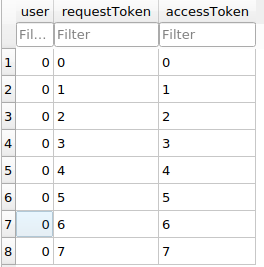
\includegraphics[width=0.5\textwidth]{figs/token1.png}
   \caption{The table of tokens showing each was associated with the user 0}
   \label{fig3}
 \end{figure}\\
This would allow all users access to user 0's account. This is a critically important vulnerability since it could be accidentally exploited by well meaning users as well as hackers.
It is also a vulnerability that requires no technical knowledge to exploit and this low skill ceiling makes it of particular threat. If combined with the fact that the bank used
to allow the transfer of money from one account to another, attackers could transfer unlimited money easily from the account of the unfortunate user whose id happens to be 0.\\ \\
\textbf{Testing the Vulnerability:} I tested this vulnerability as a hacker would by simply logging in as user 1 (which would then naturally log me in as user 0) and then
transferring money to user 1. I watched the money leave my account, which proves the issue since transferring money to myself should cause no change in value to my balance.
This would be how a hacker could exploit such a vulnerability but also how a regular user simply not paying attention and thinking they had logged into their account could also
cause trouble. This could make the vulnerability a further threat since an attacker could simply use this as an excuse if they were ever discovered to have used the attack.\\ \\
\textbf{Mitigation:} By using print lines in the \verb|getUSer()| function I discovered the issue. In the below code ids 1 and 2 in lines 1 and 2 returned 1, the correct id. This
meant that the issue was not in the fetching of the id from the database. Whilst id 3 printed 0 meaning the issue occured in the creation of the new user from the values from
the database.
\begin{minted}{java}
   System.out.println("\nID1"+rs.getInt(1));
   System.out.println("\nID2"+rs.getInt("id"));
   WondoughUser user = new WondoughUser(rs.getInt("id"),
       rs.getString("username"));
   user.setHashedPassword(rs.getString("password"));
   user.setSalt(rs.getString("salt"));
   user.setIterations(rs.getInt("iterations"));
   user.setKeySize(rs.getInt("keySize"));
   System.out.println("\nID3"+user.getID());
   return user;
\end{minted}
It then transpired that passing the id into the constructor of \verb|WondoughUser| was pointless since the constructor never set the value. Therefore I added the following line
to fix the issue.
\begin{minted}{java}
   public WondoughUser(int id, String username) {
       this.username = username;
       this.id = id;//added line
   }
\end{minted}
From here I devised an automated test to call the \verb|getUser| command to test that the user returned shared the username and id of the functions parameters.
\section{Vulnerability: Tokens are 1-10 and don't expire}
\label{sec:background}
\textbf{Description:} The access tokens on the website have 2 key issues. Firstly there are only ten eleven tokens availabe (0 through to 10). Secondly the tokens have no expiry
date and as such if a hacker were to gain access to a token through for example Javascript injection as seen in vulnerability 3, he could use it to keep permanent access to a
user's account even if they changed their password, regardless of how complex the password hashing was made. This of course is a serious security flaw and needs to be addressed.
By only having 11 tokens this flaw is made worse since an attacker would only need to try 11 tokens in order to get access. \\ \\
\textbf{Testing the Vulnerability:} To do this I logged in as \textit{hacker@wondoughbank.com} and displayed the transactions. After my fix to the login issue in the previous
vulnerability the result was identical to figure \ref{figvun6}. I then went into the developer options on my browser to display the cookies:
\begin{figure}[h]
    \centering
    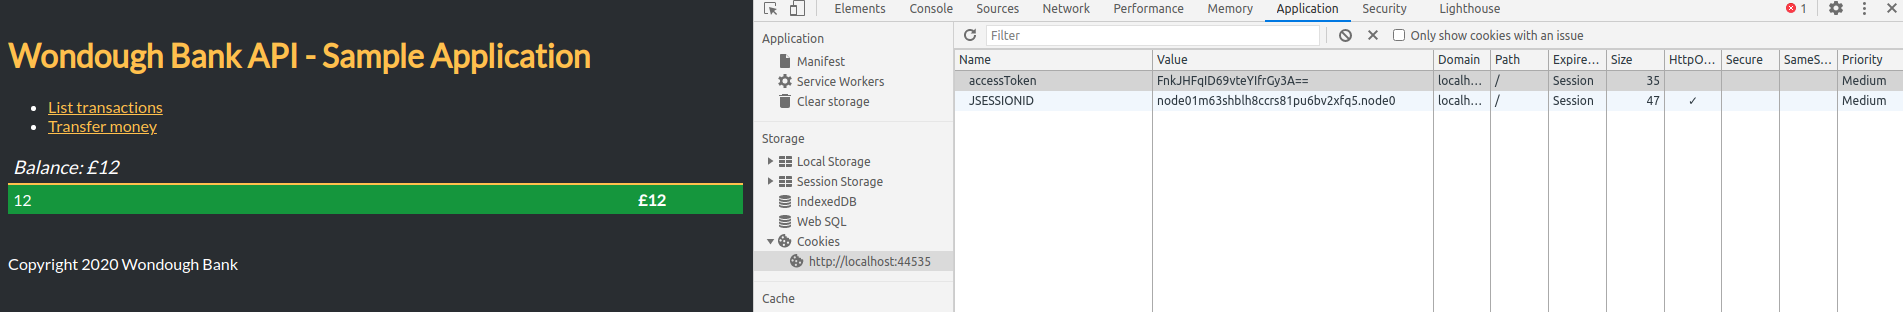
\includegraphics[width=1\textwidth]{figs/7.1.png}
    \caption{The token visible in the cookies of my session}
    \label{7.1}
\end{figure}\\
From here I was able to change the token to one associated with user 0 (from \textit{jxTkX87qFnpaNt7dS+olQw==} to \textit{jxTkX87qFnpaNt7dS+olQw==})
\begin{figure}[h]
    \centering
    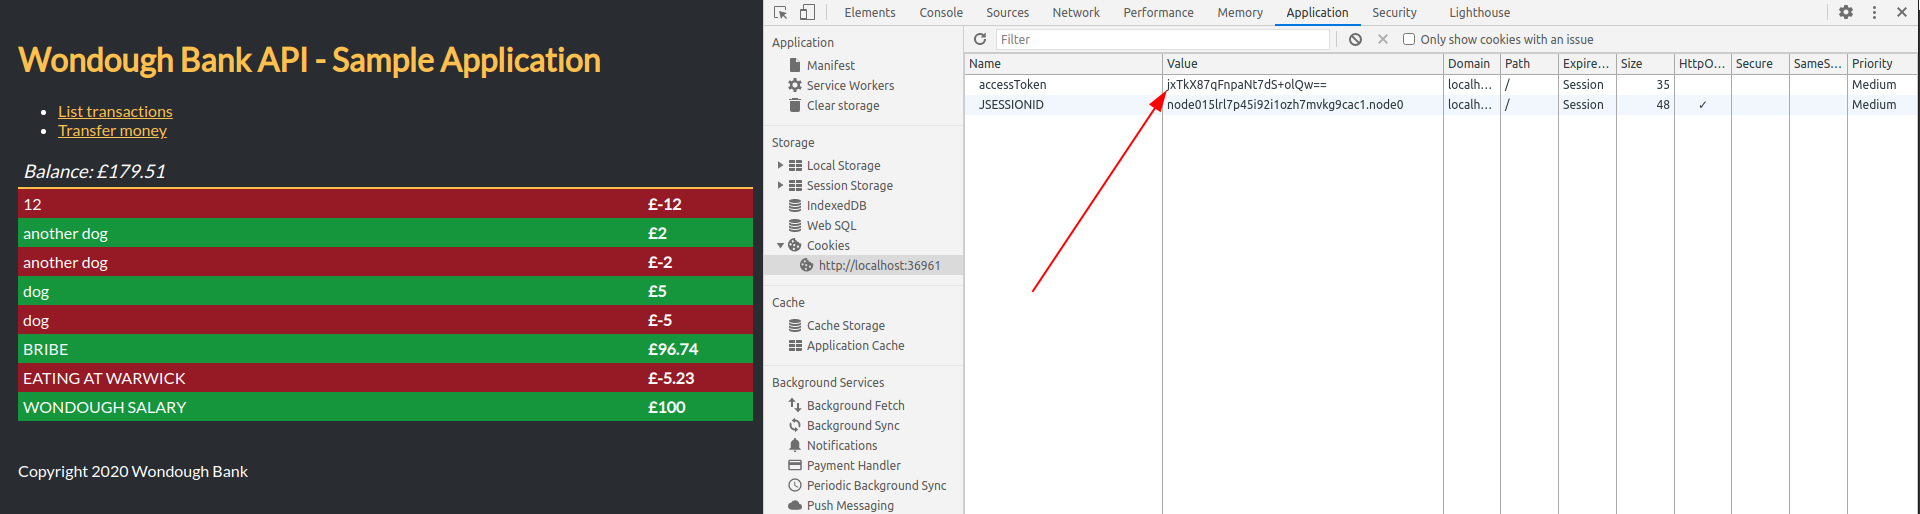
\includegraphics[width=1\textwidth]{figs/7.2.png}
    \caption{By editing the token I gain access to the intern's account}
    \label{7.2}
\end{figure}\\
\textbf{Mitigation:} The first issue of the 0-10 occurs in \verb|dbConnection| where the following code is used to create the tokens id:\\
\begin{minted}{java}
app.setRequestToken(Integer.toString(this.largestRequestToken(), 10));
app.setAccessToken(Integer.toString(this.largestAccessToken(), 10));
\end{minted}
I have therefore chosen to use the salt generation as the token since this is unique each time and much more complex. It also means that the issue of the access and request token
being the same solved.
\begin{minted}{java}
String salt;
salt = Program.getInstance().getSecurityConfiguration().generateSalt();
app.setRequestToken(salt);
salt = Program.getInstance().getSecurityConfiguration().generateSalt();
app.setAccessToken(salt);
\end{minted}
Since the salt is random each time this allows us to solve the issue of recurring tokens. To solve the issue of the fact the tokens never expire an additional column was added to
the database called \verb|expiryDate|, which was a \verb|TimeStamp| and represented the point in time when that key would no longer be valid. To set this I edited the
\verb|createApp()| function in \verb|dbConnection|. A fourth value was added to the prepared statement, which is a TimeStamp. From there the current time is stored and 30 minutes
added to it. This is to be the value of the \verb|expiryDate| of the access token. Whilst the request token has a date of 1 hour from now. The choice of times was to ensure the security
of the website was as rigorous as possible. This choice of time meant there's time to generate new access and request tokens after the access token is expired.
The request tokens will expire a little while later and can get purged in a timely manner to avoid accumulation \cite{tokens}. It also means if a hacker were to gain access to a token
it would expire shortly making access limited. However inorder to give the keys different expiry times they had to be stored seperatly, as such the function was altered to create
two entries into the database, one with request token as null and one with access token as null.
\begin{figure}[h]
    \centering
    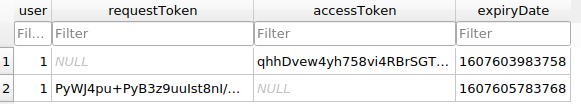
\includegraphics[width=1\textwidth]{figs/token2.png}
    \caption{The adapted way of storing tokens}
    \label{7.2}
\end{figure}\\
The expiry times were set as follows:
\begin{minted}{java}
    Timestamp now;
    now = new Timestamp(System.currentTimeMillis());
    now.setTime(now.getTime() + TimeUnit.MINUTES.toMillis(30));
    stmt.setTimestamp(4, now);

    now = new Timestamp(System.currentTimeMillis());
    now.setTime(now.getTime() + TimeUnit.HOURS.toMillis(1));
    stmt.setTimestamp(4, now);
\end{minted}
Finally a remove tokens function was created that would be called regularly to remove outdated tokens. It checked if the expiry date of the token had been surpassed by comparing
it to the current time:
\begin{minted}{java}
    long ut1 = System.currentTimeMillis();
    String query3 = "DELETE FROM authorised_apps "
                   +"WHERE expiryDate < "+ ut1 + ";";
    Statement stmt2 = this.connection.createStatement();
    int rs = stmt2.executeUpdate(query3);
\end{minted}
From this an automatic test was devised to ensure all these new criteria were met. It would create temporary tokens, ensure the difference in expiration date, value and then check
they would be removed in an hours time. The randomness and greater complecity of the tokens alongside their limited time means this vulnerability has been mitigated as far as 
possible.


\section{Vulnerability: Users cannot change their passwords}
\label{sec:background}
\textbf{Description:} The previously established issues with the salts and hashing of passwords means that we can safely assume that an attacker could easily get access to a user's
password through a combination of an sql attack with the effective use of brute forcing using rainbow tables. As such the lack of ability for a user to change their password is a
serious security flaw, since in the very real possibility that their password is discovered through the outlined techniques, it would be impossible for them or indeed Wondough to
change their password and deny the attacker further access \\ \\
\textbf{Testing the Vulnerability:} This vulnerability is much harder to test. Simply I checked each of the functions to ensure that no such command existed to update the password
of a user, which it did not. An attacker could use this exploit by using cross site scripting or sql injection (both previously outlined security flaws in this document). The use
of either vulnerability could allow the attainment of the salt, and hashed password by the attacker. As such a custom rainbow table using the salt could be created to speed up the
brute forcing process, made easier by low iterations and keysize. Once the password was obtained then the vulnerability could easily exploited by the repeated use of the password
to access the account knowing there was no way to change the password. In addition this exploit could be used by the user themselves accidentally if they happened to forget their password
and lock themselves out their account. \\ \\
\textbf{Mitigation:} I did not (in accordance with the coursework specification) do any editing to the website. Rather a function was created and rigorously tested that would update
a users password, easily implementable in a webpage at a later date. The function took three inputs, a username, a hashed current password, and a string new password. The webpage
would hash the password of the user checking it is theirs and if so directing them to this function with the new password as an input. First of all the fetches the user from the
database using \verb|getUser()| and hashes the user's new password. The function then checks if the passwords aren't the same and that the hashed password is the user's current password.
Making it only possible for someone who knows the password to change the password:
\begin{minted}{java}
WondoughUser user = getUser(username);
String newhashedPassword =
   Program.getInstance().getSecurityConfiguration().pbkdf2(newPassword,
   user.getSalt(), user.getIterations(), user.getKeySize());
if(hashedpassword.equals(newhashedPassword)) return false;
if(!(user.getHashedPassword().equals(hashedpassword))) return false;
\end{minted}
Following this if the new password is different and the old password matches the user's then a prepared statement is set up and executed to replace the password value in the database.
\begin{minted}{java}
PreparedStatement stmt;
String sql = "UPDATE users SET password =? WHERE id =?";
stmt = this.connection.prepareStatement(sql);
try{
   stmt.setString(1, newhashedPassword);
   stmt.setInt(2, user.getID());
   stmt.executeUpdate();
   return true;
}
\end{minted}
To design an automated test for this a new user was created with the password "password". Then \verb|changePassword()| is called twice, the first time with his password and the second with
the new password "password2". If the password is changed the first time the test fails as the new password must be different, and then if it doesn't change the second time it also fail.
\begin{minted}{java}
if(connection.changePassword(testuser1.getUsername(),
testuser1.getHashedPassword(), "password")) return "FAILED";
\end{minted}
Otherwise the test passed, it is then checked the two passwords are indeed different and finally the new user is removed from the database. The test passes every time, this vulnerability therefore
is mitigated.

\section{Vulnerability: Tokens are 1-10 and don't expire}
\label{sec:background}
\textbf{Description:} The access tokens on the website have 2 key issues. Firstly there are only ten eleven tokens availabe (0 through to 10). Secondly the tokens have no expiry
date and as such if a hacker were to gain access to a token through for example Javascript injection as seen in vulnerability 3, he could use it to keep permanent access to a
user's account even if they changed their password, regardless of how complex the password hashing was made. This of course is a serious security flaw and needs to be addressed.
By only having 11 tokens this flaw is made worse since an attacker would only need to try 11 tokens in order to get access. \\ \\
\textbf{Testing the Vulnerability:} To do this I logged in as \textit{hacker@wondoughbank.com} and displayed the transactions. After my fix to the login issue in the previous
vulnerability the result was identical to figure \ref{figvun6}. I then went into the developer options on my browser to display the cookies:
\begin{figure}[h]
    \centering
    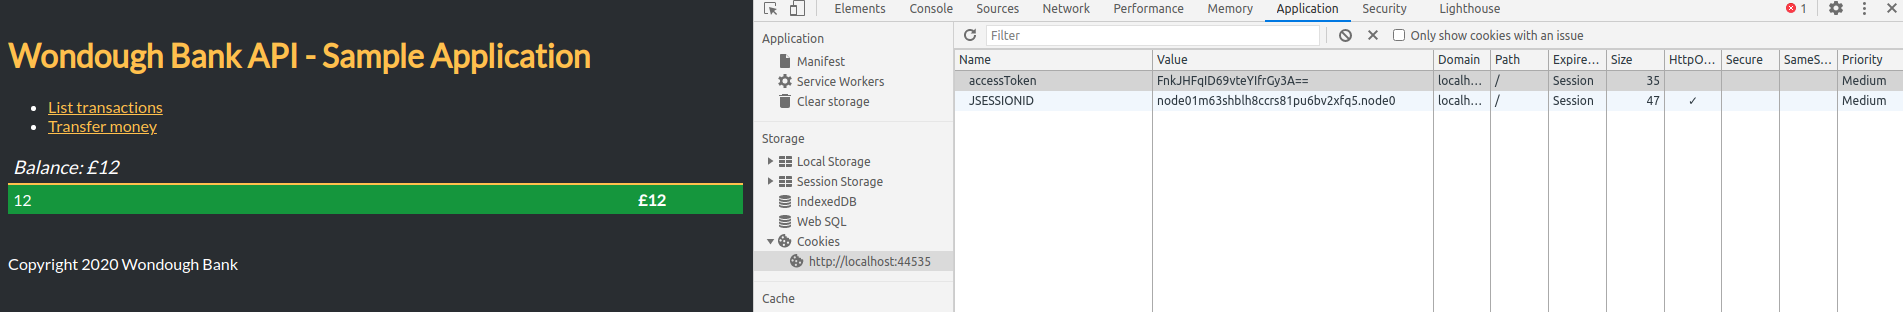
\includegraphics[width=1\textwidth]{figs/7.1.png}
    \caption{The token visible in the cookies of my session}
    \label{7.1}
\end{figure}\\
From here I was able to change the token to one associated with user 0 (from \textit{jxTkX87qFnpaNt7dS+olQw==} to \textit{jxTkX87qFnpaNt7dS+olQw==})
\begin{figure}[h]
    \centering
    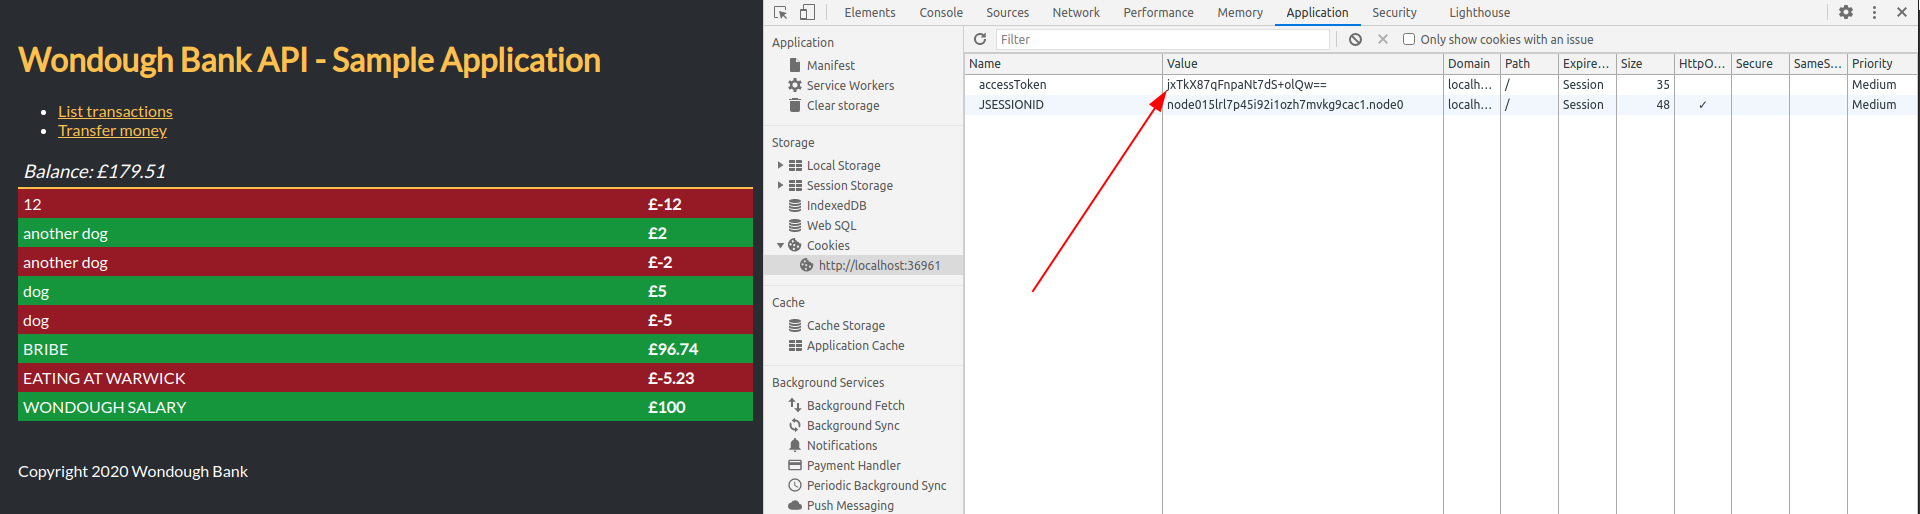
\includegraphics[width=1\textwidth]{figs/7.2.png}
    \caption{By editing the token I gain access to the intern's account}
    \label{7.2}
\end{figure}\\
\textbf{Mitigation:} The first issue of the 0-10 occurs in \verb|dbConnection| where the following code is used to create the tokens id:\\
\begin{minted}{java}
app.setRequestToken(Integer.toString(this.largestRequestToken(), 10));
app.setAccessToken(Integer.toString(this.largestAccessToken(), 10));
\end{minted}
I have therefore chosen to use the salt generation as the token since this is unique each time and much more complex. It also means that the issue of the access and request token
being the same solved.
\begin{minted}{java}
String salt;
salt = Program.getInstance().getSecurityConfiguration().generateSalt();
app.setRequestToken(salt);
salt = Program.getInstance().getSecurityConfiguration().generateSalt();
app.setAccessToken(salt);
\end{minted}
Since the salt is random each time this allows us to solve the issue of recurring tokens. To solve the issue of the fact the tokens never expire an additional column was added to
the database called \verb|expiryDate|, which was a \verb|TimeStamp| and represented the point in time when that key would no longer be valid. To set this I edited the
\verb|createApp()| function in \verb|dbConnection|. A fourth value was added to the prepared statement, which is a TimeStamp. From there the current time is stored and 30 minutes
added to it. This is to be the value of the \verb|expiryDate| of the access token. Whilst the request token has a date of 1 hour from now. The choice of times was to ensure the security
of the website was as rigorous as possible. This choice of time meant there's time to generate new access and request tokens after the access token is expired.
The request tokens will expire a little while later and can get purged in a timely manner to avoid accumulation \cite{tokens}. It also means if a hacker were to gain access to a token
it would expire shortly making access limited. However inorder to give the keys different expiry times they had to be stored seperatly, as such the function was altered to create
two entries into the database, one with request token as null and one with access token as null.
\begin{figure}[h]
    \centering
    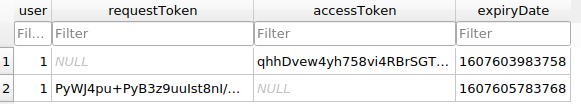
\includegraphics[width=1\textwidth]{figs/token2.png}
    \caption{The adapted way of storing tokens}
    \label{7.2}
\end{figure}\\
The expiry times were set as follows:
\begin{minted}{java}
    Timestamp now;
    now = new Timestamp(System.currentTimeMillis());
    now.setTime(now.getTime() + TimeUnit.MINUTES.toMillis(30));
    stmt.setTimestamp(4, now);

    now = new Timestamp(System.currentTimeMillis());
    now.setTime(now.getTime() + TimeUnit.HOURS.toMillis(1));
    stmt.setTimestamp(4, now);
\end{minted}
Finally a remove tokens function was created that would be called regularly to remove outdated tokens. It checked if the expiry date of the token had been surpassed by comparing
it to the current time:
\begin{minted}{java}
    long ut1 = System.currentTimeMillis();
    String query3 = "DELETE FROM authorised_apps "
                   +"WHERE expiryDate < "+ ut1 + ";";
    Statement stmt2 = this.connection.createStatement();
    int rs = stmt2.executeUpdate(query3);
\end{minted}
From this an automatic test was devised to ensure all these new criteria were met. It would create temporary tokens, ensure the difference in expiration date, value and then check
they would be removed in an hours time. The randomness and greater complecity of the tokens alongside their limited time means this vulnerability has been mitigated as far as 
possible.


\section{Vulnerability: Oauth Redirect Attack}
\label{sec:background}
\textbf{Description:} The \verb|handleAuth| function in \verb|AuthController| is used to handle \textit{Oauth} redirects to another site. This means that any site is able to use
Wondough login page as a way for their customers to login to their website. Wondough however, has no checks on the redirect addresses that are allowed to use it. As such it is
possible for the user to be redirected back to a malicious site but with an access token intended for a legitmate site. Therefore it is possible to send key information an attacker
should not have access to, through the redirecting of urls. As such the attacker who set up the malicious website an access token to gain access to the user's account of a legitmate
website. Since this websie could be anything and as such potentially very important this is a very serious secuirty flaw.\\ \\
\textbf{Testing the Vulnerability:} In order to test this I checked to see if a redirect occurs for all sites and if a token is returned. I started with the dcs website by signing
into my Wondough account under the following url.
\begin{minted}{text}
http://localhost:39476/auth?app=1&target=http://warwick.ac.uk/fac/sci/dcs/
\end{minted}
As expected I was redirected with a token. This confirmed that this vulnerability could be exploited by an attacker through a malicious website and redirect attack. I retried this
but with other websites such as \verb|www.google.co.uk|, \verb|www.amazon.co.uk| and \verb|www.bbc.co.uk|. It worked with all of them. As such it was clear that no whitelist 
existed to allow Wondough to prevent malicious sites from using this feature. \\ \\
\textbf{Mitigation:} These attacks are prevented through the use of whitelists, whereby a site will submit an application to Wondough, requesting that it's site be able to use
Wondough's login page as a way for their users to sign in. As such Wondough would be able to assess the site ensure they were happy with its legitimacy and if so then add its url
to a whitelist. As such for the purposes of fixing Wonodugh I have created a whitelist, onto which I added the Wondough website and dcs:
\begin{minted}{java}
    private static String[] safeSites
        = {"http://localhost:1464/oauth",
        "https://warwick.ac.uk/fac/sci/dcs/"};
\end{minted}
Before this I had changed the port that the client side runs on to exclusively 1464 in order to whitelist it.\\ \\
\textbf{PLEASE NOTE:} if the \textit{sample-client} is not running on port 1464 the automated test won't pass and the website will not work either.\\ \\
I then edited the \verb|handleAuth| function to only reroute whitelisted ips. To do this I created a boolean function to return whether or not the parameter was a whitelisted url:
\begin{minted}{java}
    public static boolean trustedURL(String url){
        for (int i = 0; i < safeSites.length; i++) {
            if(url.equals(safeSites[i])) return true;
        }
        return false;
    }
\end{minted}
Then in the final part of \verb|handleAuth|, the site only redirects if \verb|trustedURl| returns true for the url. Otherwise the model has an error added to it informing that the
website isn't trusted so that the user can understand why the redirect didn't go through.
\begin{minted}{java}
    if(trustedURL(getQueryLoginRedirect(request))){
        response.redirect(
        getQueryLoginRedirect(request) + "?token=" +
        URLEncoder.encode(config.md5(app.getRequestToken()), "UTF-8")
        );
    }
    else{
        model.put("error", getQueryLoginRedirect(request)
        + " isn't a trusted website");
    }
\end{minted}
The choice to use and array and create the function \verb|trustedURl| was to ensure that it was inredibly easy for Wondough to add further urls withot having to change the code. All
that is needed is for another element to be added to \verb|safeSites[]|.\\
With this issue fixed it was then necessary to devise an automted test for it. This test would make use of HTTP status codes. If wondough directed you to an external site (not localhost:1464)
the code would be 302 (wihtout the fix). This means that the client has been told to look at (browse to) another URL. Whereas after the fix the code returned upon redirection would
be 200 (Standard response for successful HTTP requests)\cite{http}. Therefore the use of \verb|httpURLConnection| was used for the test to return the status codes of a whitelisted and
non whitelisted site and ensure they were appropriate. The first part of the test initialises the connection, sets it type to \verb|POST| (so that \verb|handleAuth| is called), and sets its \verb|doOutput| to true (allowing later the sending of a request body).
\begin{minted}{java}
    URL url = new URL("http://localhost:"+ Spark.port() + "/auth?");
    HttpURLConnection con = (HttpURLConnection)url.openConnection();
    con.setRequestMethod("POST");
    con.setDoOutput(true);
\end{minted}
From here a new \verb|DataOutputStream| is declared and the value is set to the output stream of the connection. The rest of the request is then added. This includes the username, password,
appname and. This is then written using \verb|writeBytes|. Finally the status of the request is gathered and compared to its expected value.
\begin{minted}{java}
    int status = con.getResponseCode();
    con.disconnect();
    if(status != 200) return "FAILED";
\end{minted}
This is repeated for both a url from the whitelist and one not from it. If both pass the test is considered successful. The test passes everytime after the fix having failed before, thus
the vulnerability can be considered eradicated.\\ \\






\bibliographystyle{abbrv}
\bibliography{../common/bibliography}

\end{document}